\section{CAPÍTULO IV: METODOLOGÍA}\label{cap:methodology}

En este capítulo, se comenzará por discutir el diseño de la investigación para más tarde describir la metodología utilizada para conseguir cumplir los objetivos planteados en la Sección~\ref{sec:objectives}. 

Este capítulo estará en relación con el Capítulo~\ref{cap:resultsANDdiscussion} de manera que cada enfoque metodológico aportado en el presente capítulo mostrará sus resultados en el siguiente, de esta forma existirá una relación directa entre los apartados: *** 


\subsection{Diseño de Investigación}

Se ha utilizado un enfoque de investigación cuantitativa para examinar la progresión temporal de la bronquiolitis en pacientes pediátricos. De cara a alcanzar los objetivos planteados en la Sección~\ref{sec:objectives} se discutirá como la muestra limita el cumplimiento de algunos de los objetivos y frente a este límite se van a plantear diferentes alternativas. 

Como ya se ha introducido anteriormente se van a realizar $2$ estudios diferentes con distinto enfoque. A continuación se explicarán por qué se ha decidido realizar 2 estudios diferentes y se discutirán como se deben de replantear los objetivos plantados en la Sección~\ref{sec:objectives}.

Al tener 3 momentos de valoración, que son los que se muestran a continuación:

\begin{enumerate}
    \item $0$ horas $\leq$ Tiempo de Monitorización $<$ $8$ horas 
    \item $8$ horas $\leq$ Tiempo de Monitorización $<$ $16$ horas
    \item $16$ horas $\leq$ Tiempo de Monitorización $<$ $24$ horas
\end{enumerate}


Se ha plantado que se realicen valoraciones del paciente monitorizado antes de terminar el intervalo de monitorización. Es decir que al final de las $8$, $16$ y $24$ horas, se valore si: 

\begin{itemize}
    \item ¿El paciente va a necesitar OAF?
    \item ¿El paciente necesitará ser ingresado en la UCIP?
\end{itemize}

Existe un factor limitante a la hora de hacer estos $3$ estudios predictivos.

En primer lugar es la falta de datos de pacientes que han ingresado en la UCIP. Si se parte de los pacientes válidos; \texttt{Valid\_patients\_P1}, definidos en la Sección~\ref{sec:seleccion_pacientes}, que son aquellos que muestran un porcentaje de valores faltantes menor del $5\%$ en las primeras $24$ horas de monitorización, se puede ver cómo solo $4$ han sido llevados a la UCIP, por el contrario existe un mayor registro de pacientes que han necesitado soporte respiratorio mediante el uso de la OAF, $14$. Esta distribución de pacientes se muestra en la Figura~\ref{fig:bar-OAF-UCIP-valid-1} de a continuación: 

\begin{figure}[H]
    \centering
    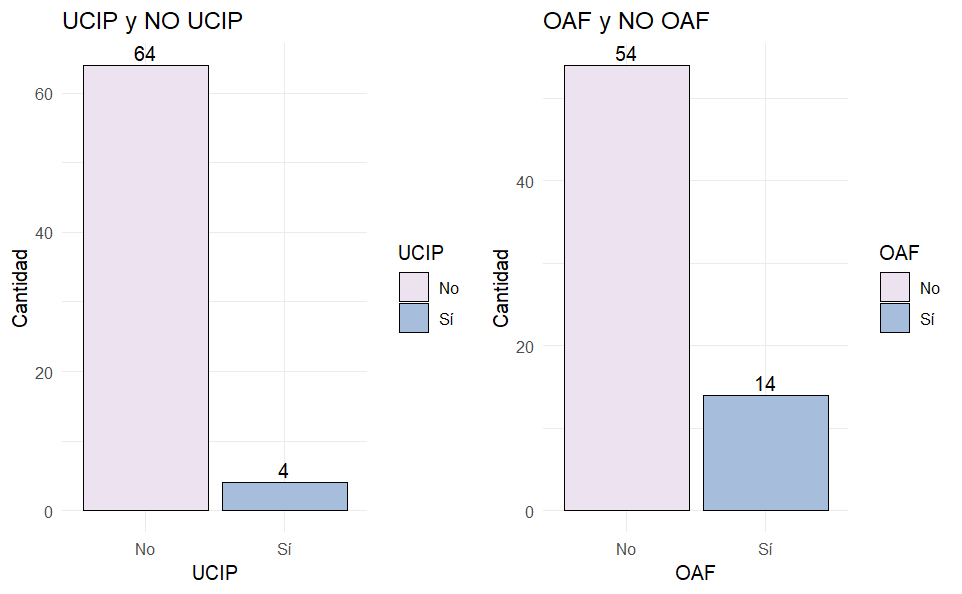
\includegraphics[scale = 0.9]{./img/bar-OAF-UCIP-valid-1.png}
    \caption{Cantidad de pacientes que han sido trasladados a la UCIP y los que NO, que han necesitado OAF y lo que NO, del conjunto de pacientes válidos: \texttt{valid\_patient\_1}}
    \label{fig:bar-OAF-UCIP-valid-1}
\end{figure}

De cara a plantear la investigación teniendo en cuenta los diferentes intervalos antes mencionados, es necesario ver la distribución de los pacientes dentro de los mismos. Esto se puede ver a continuación en la siguiente Figura~\ref{fig:intervalos-valid-1}.

\begin{figure}[H]
    \centering
    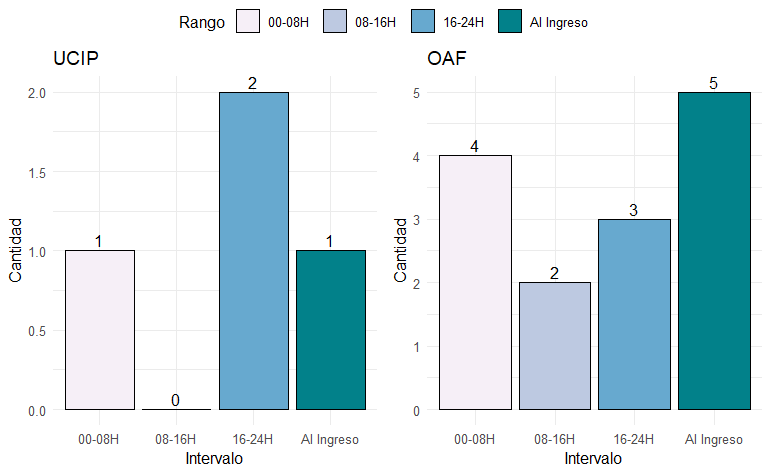
\includegraphics[scale = 0.9]{./img/intervalos-valid-1.png}
    \caption{Distribución de los pacientes dentro de los $3$ intervalos de estudio del conjunto de pacientes: \texttt{valid\_patient\_1}}
    \label{fig:intervalos-valid-1}
\end{figure}


Una vez vista la distribución de los pacientes que presentan UCIP y OAF en los $3$ intervalos de tiempo antes mencionados, cabe preguntarse si tiene sentido plantear el presente trabajo de la forma previamente discutida.

Respecto a los pacientes que son ingresados en la UCIP, se les va a catalogar como pacientes que han sufrido un \textit{Deterioro}. Dado que todos los pacientes que han sido ingresados en la UCIP han recibido soporte respiratorio mediante la técnica OAF, simplemente se les va a considerar como pacientes que han necesitado OAF. En otras palabras, no se utilizará la variable UCIP como variable de salida en este trabajo debido a la escasa representación de este tipo de paciente. Esta consideración se ha mencionado anteriormente en el conjunto total de pacientes en la Figura~\ref{fig:venn-OAF-UCIP} de la Sección~\ref{sec:seleccion_pacientes}.

La exclusión de los pacientes que han sufrido OAF tiene sentido, ya que una vez que al paciente se le suministra OAF, los datos de monitorización recogidos del mismo ya están afectados por la técnica de soporte respiratorio. Por lo tanto, carece de sentido utilizar dichos datos para predecir si el paciente va a necesitar OAF en las próximas $8$ horas, ya que se están recogiendo en un contexto diferente al de los demás pacientes.

Respecto a los pacientes que se les ha aplicado OAF, si excluimos a los pacientes que se les ha aplicado OAF nada más ser ingresados, y aquellos que la han necesitado en las primeras $8$ horas, solo nos quedan 5 pacientes del conjunto de pacientes que han sufrido OAF para realizar el estudio. La falta de presencia de pacientes de este conjunto se va a abordar mediante la técnica de \textit{oversampling-SMOTE} que se explicará en la Sección~\ref{sec:oversampling}.

Una vez explicado el motivo de la exclusión de los pacientes que han sido ingresados en la UCIP y los que han necesitado OAF, se va a proceder a explicar los $2$ estudios que se van a realizar en la Sección~\ref{sec:estudios}.

\subsubsection{Estudios}\label{sec:estudios}

\paragraph{Estudio 1}\label{sec:estudio1}

En el \textit{Estudio 1} se considerará al conjunto de pacientes: \texttt{Valid\_patients\_P1}. En este estudio se pretende observar las posibles diferencias entre las \textit{Series Temporales} de monitorización en función de si el paciente ha sido intervenido con OAF o no. Para ello se va a realizar un análisis ANOVA de las medias de las variables de monitorización (\textit{Frecuencia Cardiaca} y \textit{Saturación de O$_2$}) de los pacientes que han necesitado OAF y los que no.

\paragraph{Estudio 2}\label{sec:estudio1}

En el \textit{Estudio 2} se considerará el conjunto de pacientes: \texttt{Valid\_patients\_P2}. En este estudio se pretende observar si es posible predecir si un paciente va a necesitar OAF en las próximas $8$ horas al ingreso. 

Antes de realizar el modelado del algoritmo de clasificación discreta se va a querer visualizar si mediante el \textit{clustering} de los valores de monitorización de los pacientes se pueden observar diferencias entre los pacientes que han necesitado OAF y los que no. Para la correcta ejecución de lo anteriormente mencionado se seguirán varios pasos:

\begin{enumerate}
    \item \textbf{Selección de Datos:} Al tener 480 valores de monitorización de \textit{Frecuencia Cardíaca} y \textit{Saturación de O$_2$} se van a utilizar diferentes datos para la ejecución de los clusters:
    \begin{enumerate}
        \item \textsc{Datos en bruto:} Se van a utilizar los 480 datos en bruto de monitorización de los pacientes de cada \textit{Serie Temporal}.
        \item \textsc{Función de autocorrelación (FAC):} Se van a utilizar las primeras 50 observaciones de la FAC de cada \textit{Serie Temporal}.
        \item \textsc{Función de autocorrelación cruzada (FACC):} Se van a utilizar las primeras 100 observaciones de la FACC de la relación entre las \textit{Serie Temporales} de \textit{Frecuencia Cardíaca} y \textit{Saturación de O$_2$}.
        \item \textsc{Periodograma:} Se usarán los periodogramas de cada \textit{Serie Temporal}.
    \end{enumerate}
    
    \item 
\end{enumerate}


Para ello se va a realizar un análisis de clasificación binaria, donde la variable de salida será si el paciente ha necesitado OAF o no. Para ello se van a utilizar los datos de monitorización de las primeras $8$ horas de monitorización de los pacientes.











\subsubsection{Oversampling}\label{sec:oversampling}

En el campo médico, suele ser común encontrarse con conjuntos de datos donde una categoría tiene significativamente menos observaciones que otra, es decir el conjunto total de la muestra se presenta desbalanceada. Esta disparidad puede afectar negativamente el rendimiento de los modelos de clasificación, ya que pueden tener dificultades para aprender patrones de la clase minoritaria. En el caso de este estudio dónde solo se cuenta con solo 5 pacientes en una categoría (paciente que ha necesitado OAF posteriormente a las $8$ primeras horas de ingreso) y 40 (paciente que no ha necesitado OAF) de la  otra, existe un claro desequilibrio que puede impactar la precisión de cualquier modelo que se intenta construir.

La técnica utilizada en este trabajo, SMOTE (Synthetic Minority Over-sampling Technique) es un algoritmo estadístico utilizado para abordar el problema de muestras desbalanceadas en datos de clasificación. En lugar de simplemente duplicar las observaciones de la clase minoritaria, SMOTE crea nuevas muestras artificiales interpolando entre observaciones cercanas. Esto se logra eligiendo una observación de la clase minoritaria y generando puntos artificiales en la dirección de sus vecinos más cercanos de la misma categoría. De esta manera, se aumenta el número de observaciones de la clase minoritaria sin simplemente duplicar los mismos puntos (~\cite{Chawla2002}).

















Una vez pasadas las $8$ primeas horas se pretende valorar si el paciente va a necesitar OAF en las próximas $8$ horas y así sucesivamente. Partiendo de esta situación el objetivo sería que dentro de las primeras $24$ h de ingreso del paciente se le valore en $3$ momentos con qué porcentaje va a necesitar OAF en las $8$ horas siguientes. De cara a plantear esta metodología para este estudio existe el factor limitante de la muestra de pacientes con la que se trabaja, dónde la mayoría de pacientes no sufren OAF y por tanto no se puede realizar un estudio de este tipo dónde se divide por intervalos a la muestra de pacientes que sufren OAF. A continuación, se muestra en relación al conjunto de pacientes \texttt{Valid\_patients\_P1} cómo se distribuyen los pacientes que han necesitado OAF en los distintos intervalos:

En este estudio este planteamiento se muestra limitado puesto que más de la mitad de pacientes que se han considerado válidos para el estudio (según el criterio valid\_patient\_2 adoptado en el apartado ***) que necesitan OAF la requieren al ingreso o en las primeras 8 horas (De los 16 pacientes válidos que presentan deterioro 10 pacientes; 5 al ingreso y 5 antes de las 8 primeras horas). Esto supondría eliminar de la ecuación estos 10 pacientes y solo tener en cuenta a los 6 restantes para valorar las 8 primeras horas y solo a 2 para valorar las 16 primeras.



\begin{itemize}
    \item El primer estudio, \textit{Estudio 1}, como se ha tratado anteriormente en la Sección~\ref{sec:metodologias_exclusion_pacientes} de selección de pacientes válidos para los distintos estudios, se va a centrar en el estudio de todos los pacientes pediátricos considerando las primeras $24$ horas desde el ingreso. En este caso se valorará de manera general la evolución de los pacientes y diferencias entre aquellos que se les ha intervenido con OAF y los que no. En este estudio simplemente se tendrán en consideración las variables \textit{Series Temporales} referenciadas en la tabla~\ref{tabla:variables_estudio} y se realizará un estudio descriptivo de las mismas.
    \item  En el segundo estudio, \textit{Estudio 2}, se valorará la evolución de los pacientes que han necesitado OAF y se comparará con los que no han necesitado OAF para así poder generar un modelo que permita predecir si un paciente va a necesitar OAF o no en las siguientes próximas horas. Es este estudio se pretenderá realizar un modelo que permita prever la necesidad de OAF en las 8 h de ingreso. ad de OAF en las horas siguientes de las 
\end{itemize}

Se utilizarán aquellas variables que se han definido anteriormente en la Sección~\ref{sec:tiposdevariables} y en concreto de aquellas recogidas en la Tabla~\ref{tabla:variables_estudio}:

\begin{itemize}
    \item Descriptivas dentro del \textit{scope} del estudio.
    \item Temporales en $3$ Intervalos dentro del \textit{scope}.
    \item Series Temporales.
\end{itemize}

Las variables utilizadas e el \textit{Estudio 2} será menos que las usadas en el \textit{Estudio 1}

ha partido de 47 variables descriptivas y de 2 variables que muestran la evolución temporal de los pacientes durante las primeras 24 h de ingreso y que han sido tratadas en el presente trabajo como series temporales. 


Explicación de los distintos Estudios:


En el caso del Estudio 2:

Idealmente 



\begin{figure}[H]
    \centering
    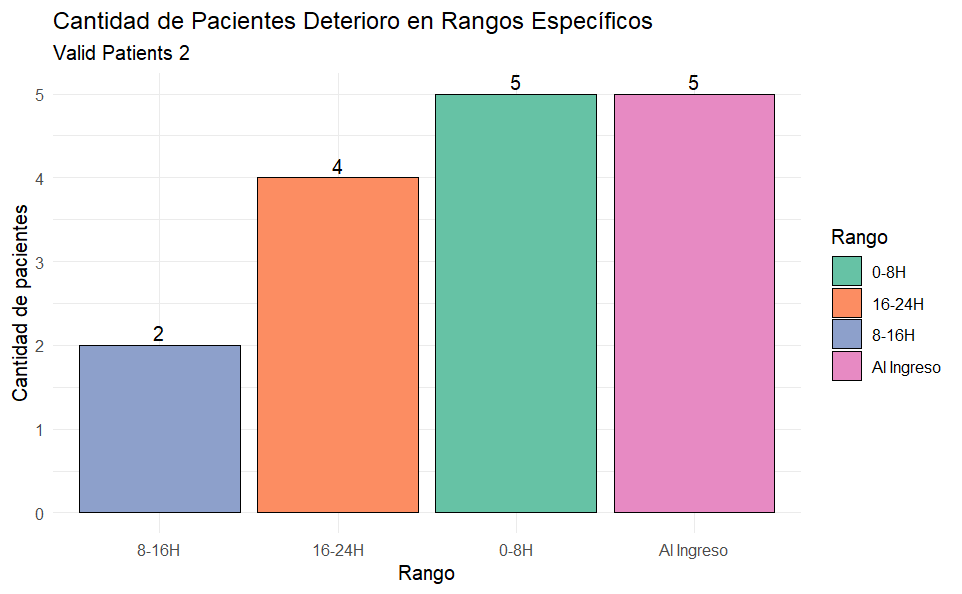
\includegraphics[scale = 1]{./img/bar-deterioro-valid-2.png}
    \caption{Cantidad de Pacientes Deterioro en Rangos Específicos de Tiempo considerando solo los pacientes sgún criterio valid\_patient\_2}
    \label{fig:bar-deterioro-valid-2}
\end{figure}

Se va a separar entre pacientes que han necesitado OAF al ingreso y los que no.

A continuación se muestran en rojo aquellos pacientes que a pesar de haberles suministrado OAF han necesitado ser trasladados a UCIP.

En contraposición se muestran en verde aquellos pacientes que han necesitado OAF pero no han necesitado ser trasladados a UCIP. 



Ningún paciente cómo ya se ha visto ha necesitado traslado a UCIP sin haber necesitado OAF previamente.

